\chapter{Frontend electronic of the scintillating fiber hodoscope}\label{cha:frontend}
%the sidevieve hast to be updates
%citroc picute has to be included ans described witharrowas and refreces to the figure have to be included in the text
\section{Overview of the frontend electronics}
\begin{figure}[h]
    \centering
    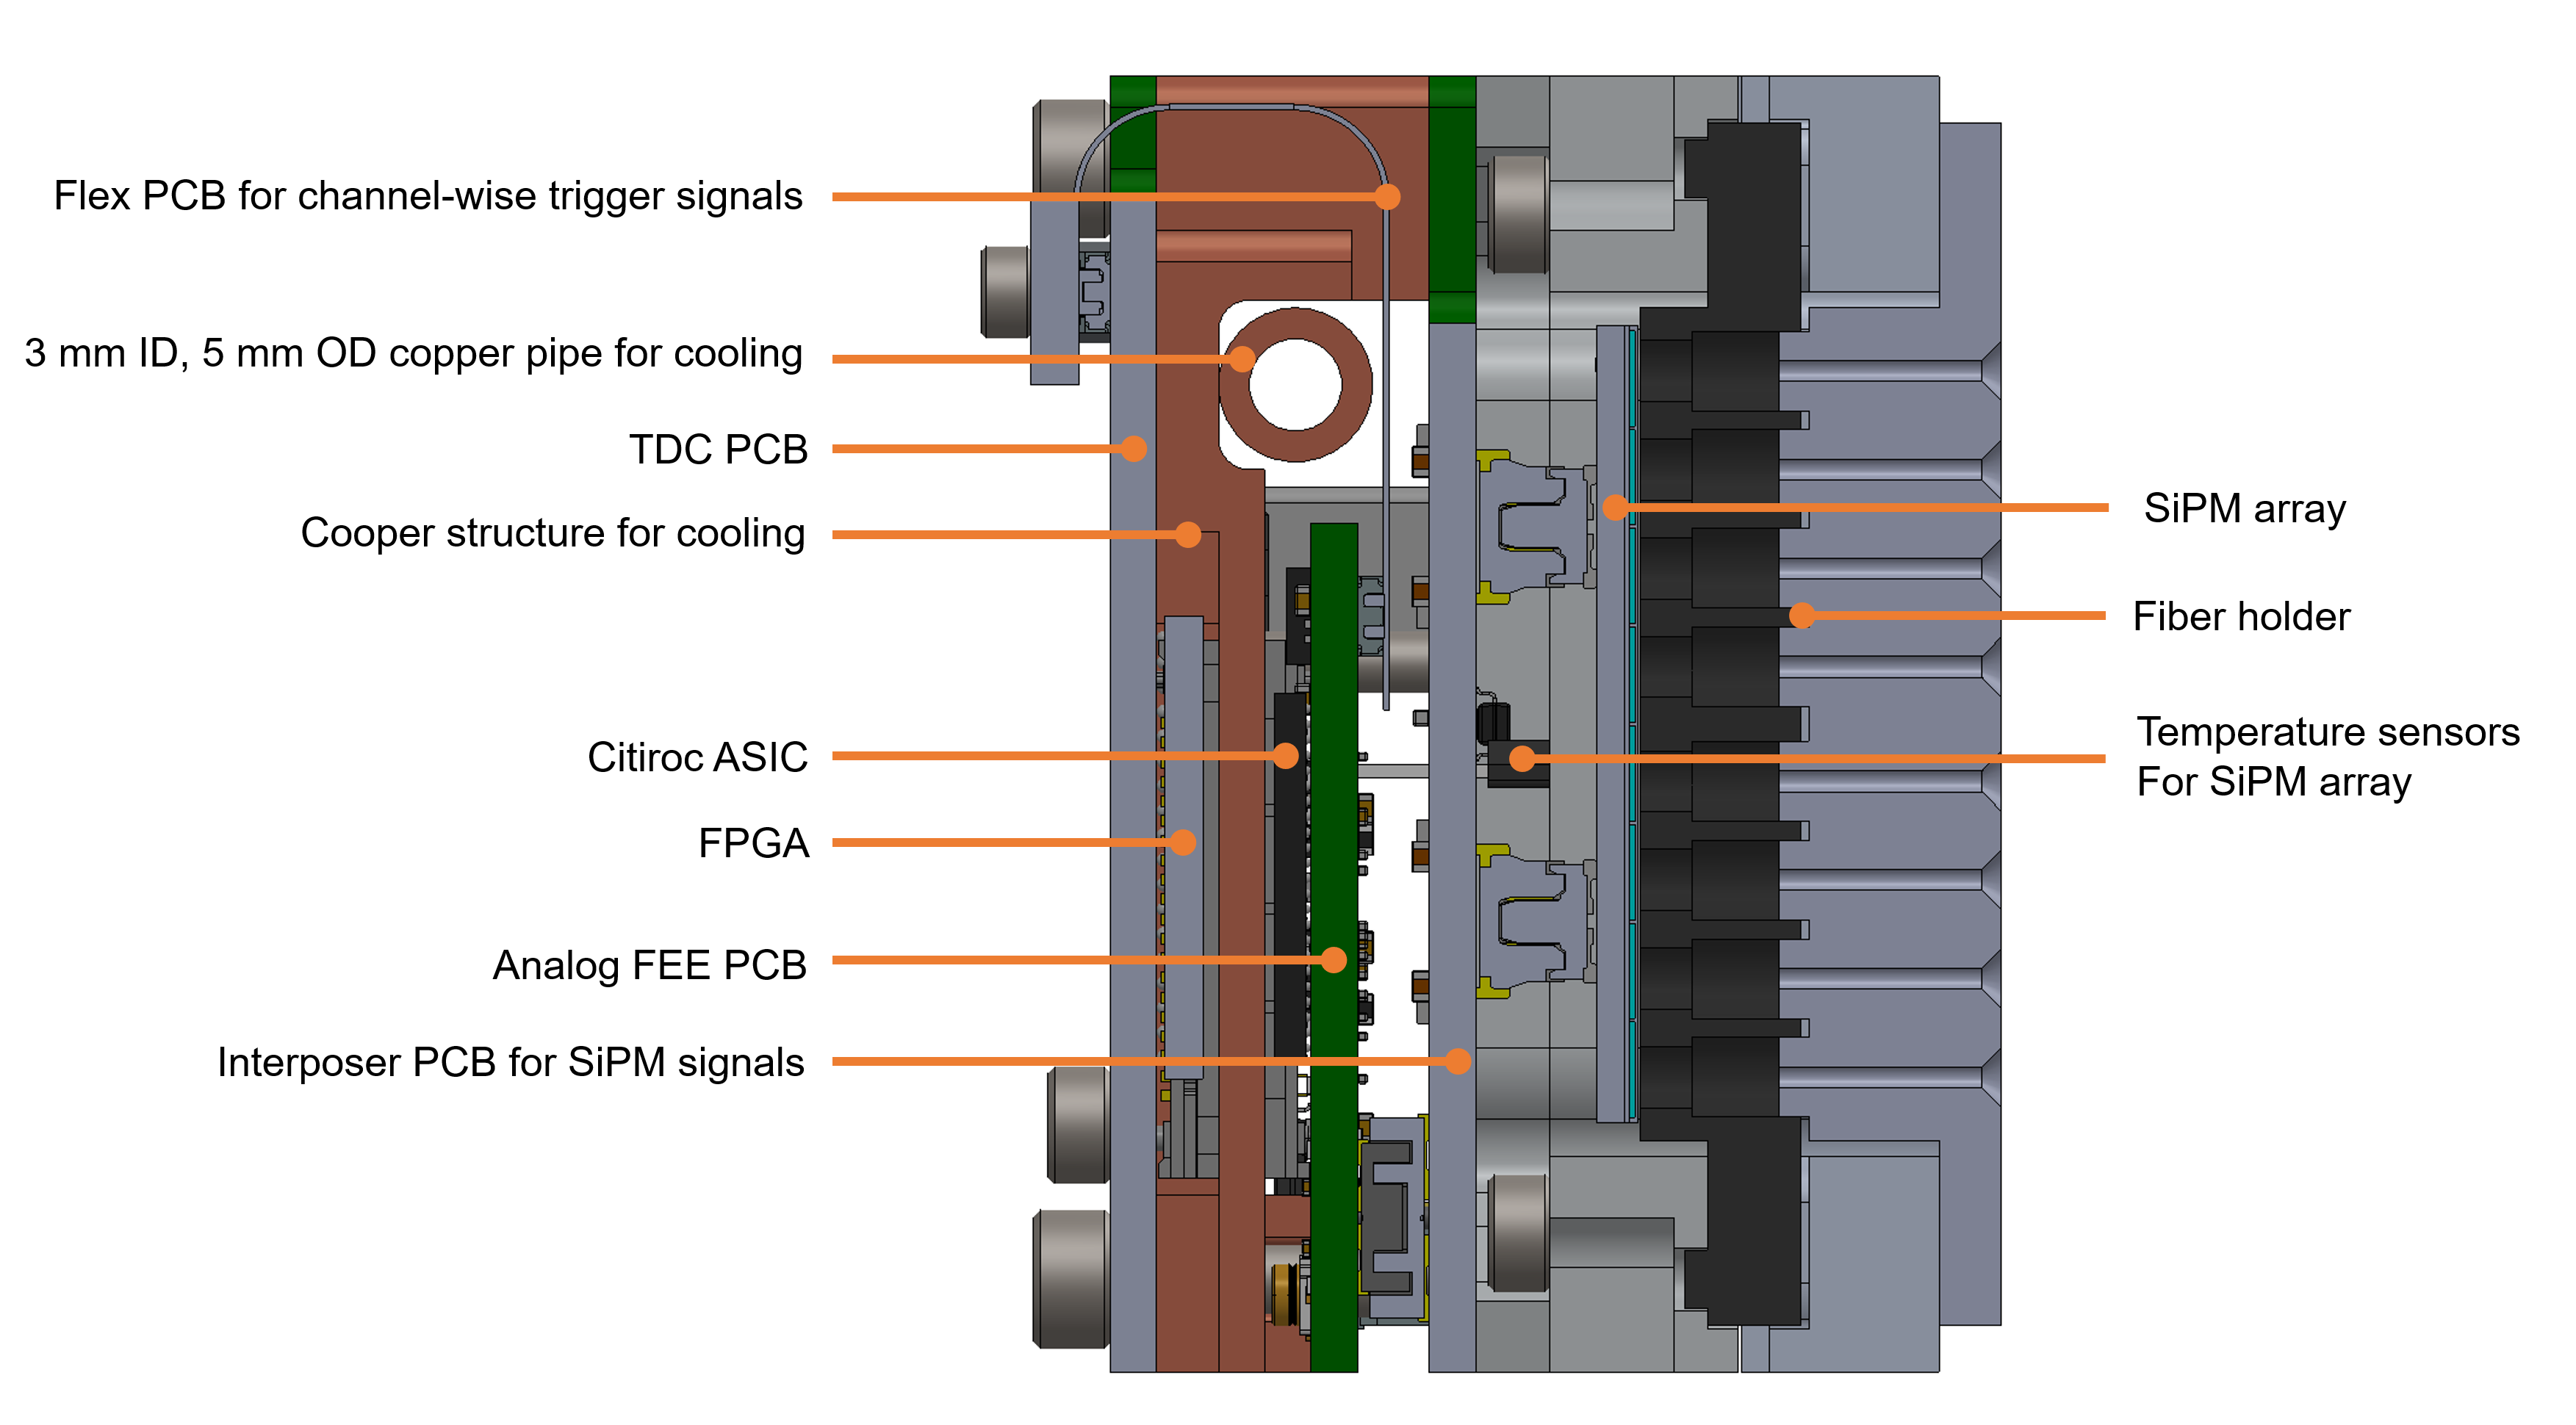
\includegraphics[width=0.9\textwidth]{SideViewElectronics.PNG}
    \caption{Sideview of the frontend electronics that will be attached on the sides of the SFH, the fiber holders will be attached to the fibers.
     The SiPM arrays transform the incoming photons into  electric signals that are then transferred to the frontend electronics by the PCB interposer.\autocite{InternalcommunicationKarl}}
    \label{fig:SideviewModelElectronics}
    \end{figure}
\subsection{Proccesing of the SFH signal}
The frontend electronics of the scintillating fiber hodoscope process the signals from the scintillating fibers.
They can be attached on all four sides of the SFH, as can be seen in figure \ref{SFHpicture}.
The fibers are conected to the fiber holders on both ends as shown in figure \ref{fig:SideviewModelElectronics}. 
There are in total 768\autocite{Amber2022Status} fibers per SFH. Since both ends produce an electric signal,
 a total of 1546 signals or 384 signals, for every attached electonics unit have to be proccesed.
 \newline
 The incoming photons are transformed into electric signals by the SiPM arrays.
 The SiPM signals are then transmitted to the analog frontend electronics (FEE) PCB by the interposer PCB also shown in figure \ref{fig:SideviewModelElectronics}.\autocite{InternalcommunicationKarl}
\subsection{The analog frontend electronics (FEE) PCB}
\begin{figure}[H]
    \centering
    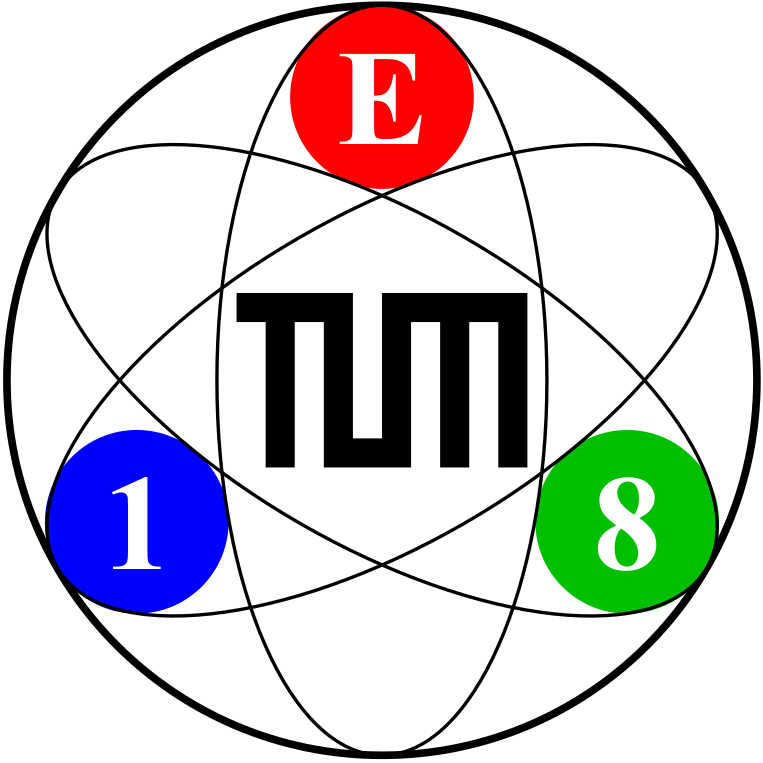
\includegraphics[width=0.6\textwidth]{E18Logo.PNG}
    \caption{The analog frontend electronics (FEE) PCB with the six CITIROC1A ASICs, on the left cite you can see the region where the power supply is connected.The output of the CITIROC1A is transmitted to the iFTDC over three flex PCBs.\autocite{InternalcommunicationKarl}}
    \label{fig:FEE}
\end{figure}
The analog frontend electronics (FEE) PCB, shown in figure \ref{fig:FEE}, together with the iFTDC form the heart of the frontend electronics.
It contains six CITIROC1A ASICs, which are used to amplify and process the signals,32 by each CITIROC1A ASIC , from the SiPM arrays.The output of the CITIROC1A is then transmitted to the iFTDC over three flex PCBs.
The power supply is connected to the FEE PCB on the left side.Two CITIROC1A ASICs are each controlled by one Artix-7 FPGA located on the iFTDC.\autocite{InternalcommunicationIgor}
\subsection{The iFTDC}
\begin{figure}[H]
    \centering
    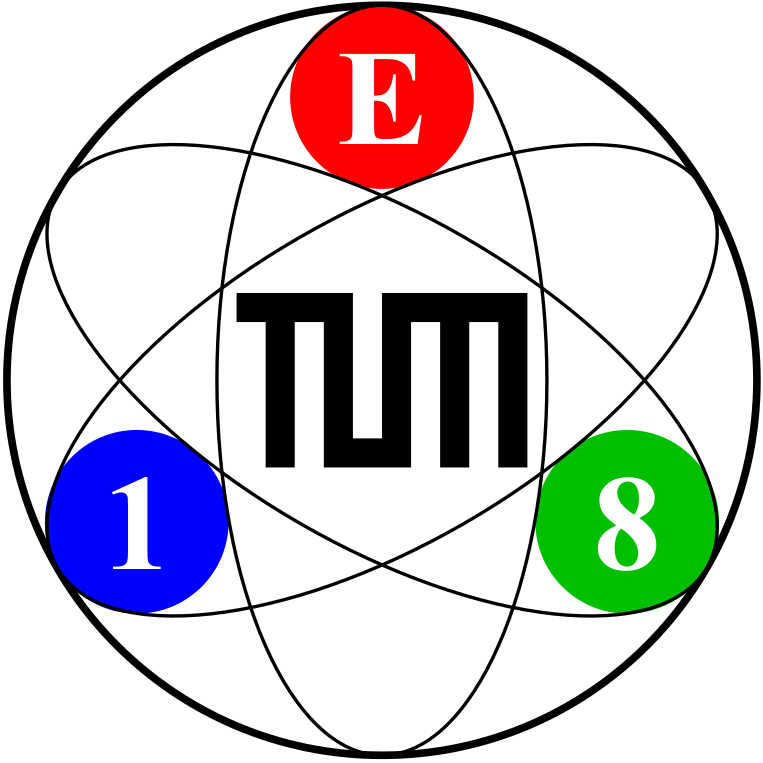
\includegraphics[width=0.6\textwidth]{E18Logo.PNG}
    \caption{The iFTDC with three Artix-7 FPGA, the three flex PCBs that connect the iFTDC with the FEE PCB and the power supply.\autocite{InternalcommunicationIgor}}
    \label{fig:iFTDC}
\end{figure}

The iFTDC is a FPGA based time-to-digital converter depicted in figure \ref{fig:iFTDC}.It is made up out of three Artix-7 FPGA, who each control two CITIROC1A ASICs.
The FPGA handels the readout as well as the configuration of the CITIROC1A ASICs\autocite{InternalcommunicationIgor}.
The focus of this thesis is the devolopment of FPGA firmware for the configuration of the CITIROC1A ASICs, but a provisional readout firmware will also be developed.
\newline
INSERT: here stil hast to be includes how ethernet works how ipbus works and how jtag is implemented ans stuff analong this line 
\section{The CITIROC1A ASIC}
